\documentclass{beamer}

\mode<presentation>
{
  \usetheme{default}      % or try Darmstadt, Madrid, Warsaw, ...
  \usecolortheme{default} % or try albatross, beaver, crane, ...
  \usefonttheme{default}  % or try serif, structurebold, ...
  \setbeamertemplate{navigation symbols}{}
  \setbeamertemplate{caption}[numbered]
} 

\usepackage[french]{babel}
\usepackage[utf8x]{inputenc}
\usepackage{fancyvrb}
\usepackage{graphicx}

\author{David Wong
  \and Jacques Monin
  \and Hugo Bonnin}

\title{Implémentation et Analyse d'une White-box du DES}

\institute{Université de Bordeaux}

\date{2014}

\begin{document}

\begin{frame}
  \titlepage
\end{frame}

\begin{frame}{Plan}
  \tableofcontents
\end{frame}

\section{A quoi ça sert ?}

\begin{frame}{A quoi ça sert ?}
  \begin{itemize}
  \item Nouveau concept
  \item Loin d'être parfait
  \end{itemize}
\end{frame}

\subsection{Man In The Middle}

\begin{frame}{Base de la cryptographie}

  \begin{figure}[h]
    \centering
    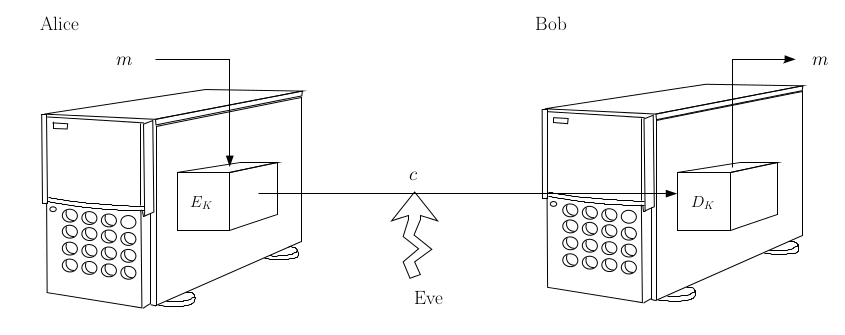
\includegraphics[scale=0.50]{./images/alice_bob.png}
    \caption{Man In The Middle}
    \label{fig:keygen}
  \end{figure}

\end{frame}

\subsection{Man At The End}

\begin{frame}{Man At The End}
  
\end{frame}

\subsection{Exemples}

\begin{frame}{Exemples}

 \begin{figure}[h]
    \centering
    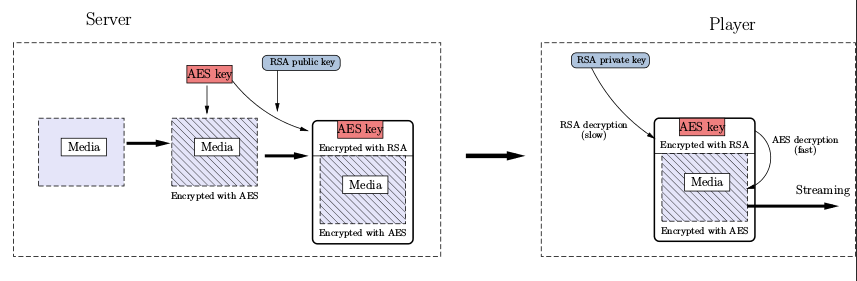
\includegraphics[scale=0.50]{./images/drms.png}
    \caption{DRMs}
    \label{fig:keygen}
  \end{figure}

\end{frame}

\section{Whitebox}

\subsection{Définition}

\begin{frame}{Définition}

  \begin{figure}[h]
    \centering
    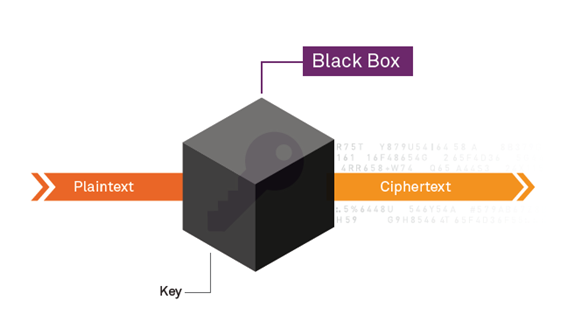
\includegraphics[scale=0.30]{./images/blackbox.png}
    \caption{Cas typique}
    \label{fig:keygen}
  \end{figure}

  \begin{figure}[h]
    \centering
    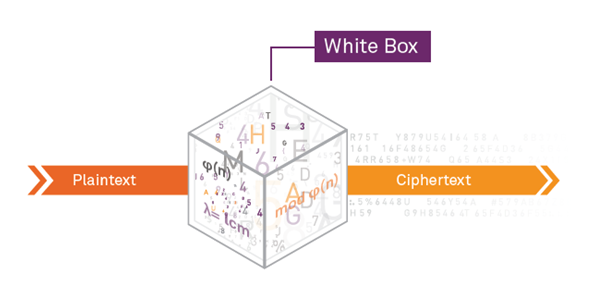
\includegraphics[scale=0.30]{./images/whitebox.png}
    \caption{Nouveau cas}
    \label{fig:keygen}
  \end{figure}

\end{frame}

\subsection{DES}

\subsection{Github}

\section{Concepts}

\subsection{Partial Evaluation}

\subsection{Tabularization}{Tabularization}

\begin{frame}[fragile] 

\begin{Verbatim}[samepage=true]
       .----.     .-------------------.     .----.
       |    |     |                   |     |    |
       |    |     |                   |     |    |
       |    |     |                   |     |    |
       | Y0 |  =  |         M         |  x  | X0 |
       |    |     |                   |     |    |
       |    |     |                   |     |    |
       |    |     |                   |     |    |
       '----'     '-------------------'     '----'

       .----.     .----.----.----.----.     .----.
       |    |     |    |    |    |    |     | X0 |
       | Y0 |     | A  | B  | C  | D  |     .----|
       |    |     |    |    |    |    |     | X1 |
       .----.  =  .----.----.----.----.  x  .----.
       |    |     |    |    |    |    |     | X2 |
       | Y1 |     | E  | F  | G  | H  |     .----.
       |    |     |    |    |    |    |     | X3 |
       '----'     '----'----'----'----'     '----'
\end{Verbatim}

\end{frame}

\subsection{Input/Output Encoding}

\begin{frame}
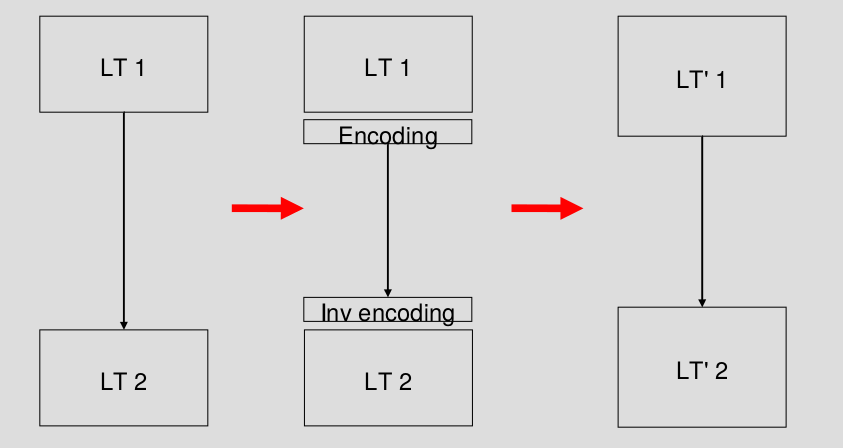
\includegraphics[scale=0.50]{images/encoding.png}
\end{frame}

\section{Concepts secondaires}

\subsection{Randomization}

\subsection{Mixing Bijection}

\subsection{Bypass}

\subsection{Combined Function Encoding}

\subsection{Split-Path Encoding}

\subsection{External Encoding}

\section{Conclusion}


\end{document}
